% This is the first draft of MMU Faculty of Engineering Cryptography and Security systems assignment
% for 18/19 Trimester 2
% Chia Jason 1161300548
% Hor Sui Lyn 1161300122
%
\documentclass[runningheads]{llncs}
\usepackage{graphicx}
\usepackage[margin=0.8in]{geometry}
\usepackage{titlesec}
\usepackage{float}
%
\begin{document}

% title
\title{The Technology of Virtual Machine Monitors and Architectural Support for VM Operating Systems}
%\thanks{Supported by Mult x.} % if we want to thank someone/org.
%
% authors
\author{Rishi Ranjan, Amish Garg, Tanav Shah, Nihal Choudhary, Saurav Pandit, Om Katiyar, Shubhrat Agarwal }
%
\maketitle              % typeset the header of the contribution
%
%
%
%
\section{Introduction}
\subsection{Abstract Idea of Virtualization}
\large A virtual-machine monitor (VMM) enables creation. management and governance of Virtual Machines on top of a physical host machine. VMM manages the backend operation of VMs by allocating the necessary computing, memory, storage and other I/O resources. A few simple extensions to a host operating system can make it a much faster platform for running a VMM. This project deals with the architectural support for virtualization running over a host OS. Virtualization today is mainly handled by hypervisor technology. Here we look at how the architecture of a system can support the security of a virtual machine, memory isolation for the VM and hybrid virtualization of the VMs.

\subsection{Modules present in the Project}
1. Introduction to Virtual Machines and VMMs\newline
2. Host OS Support for VMs\newline
3. ARM architecture Support for VMs\newline
4. Hosted Virtual Machine Architecture\newline
5. Network Performance\newline
6. Security Flaws in VMs\newline
7. MIPS support

\subsection{Relevance of the idea}
 Virtualization today is very relevant in the computing world because it allows for a system to run multiple OS even with its limited hardware resources. It allows for parallelization of tasks, ease of running an OS and what not. In today’s world safer servers and data centers have their future in virtualization itself.

%
%
\section{Description of the modules}
\subsection{Introduction to VMMs}
As defined by IBM, a “Virtual Machine” is a fully protected and isolated copy of the underlying physical machine’s hardware. A virtual machine can be used in place of having a dedicated physical machine to write and test programs without crashing physical machine.
A software layer called a virtual machine monitor (VMM) controls the machine hardware. Every virtual machine is created by the VMM and behaves like a complete physical machine having its own dedicated operating system.
The monitor is the interaction layer between the Virtual Machines and Physical Machine. It gets out of the way whenever possible to allow virtual machine to interact directly with the hardware consequently maximizing performance. This direct execution property allows mainframe-class virtual machines to achieve close to native performance and sets the technology apart from machine emulators that always impose an extra layer of terpretatuin on the emulated machine.

\begin{figure}[H]
 
      \centering
     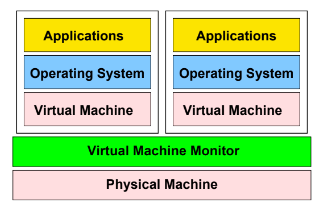
\includegraphics[width=50mm,height=50mm]{virtual_machine_organisation.png}
     \caption{Penalty Index Comparison}
     \label{fig:galaxy}
  
 \end{figure}

Reference [1]

[1] Title : Virtualizing I/O Devices on VMware Workstation’s Hosted Virtual Machine Monitor
    Authors: Jeremy Sugerman, Ganesh Venkitachalam and Beng-Hong Lim

\subsection{Host OS support for VMs}
UMLinux is Type II VMM, the guest operating system and the guest applications all run as a single process on a host Linux OS. It provides a higher-level interface to the guest OS that is similar to underlying hardware.

Bottlenecks:
UMLinux’s system structure with two separate host processes causes an inordinate number of context switches on the host.
Switching between the guest kernel and the guest user space generates a large number of memory protection operations.
Switching between two guest application processes generates a large number of memory mapping operations.\newline
Solution:
Most of these context switches can be eliminated by moving the VMM process’s functionality into the host kernel. We encapsulate the bulk of the VMM process functionality in a VMM loadable kernel module. Moving the VMM process’s functionality into the host kernel drastically reduces the number of context switches in UMLinux\newline
Our first solution protects the guest
kernel space from guest user code by changing the bound on
the user code and data segments .When the guest-machine
process is running in guest user mode, the VMM kernel
module shrinks the user code and data segments to span
only [0x0, 0x70000000). When the guest-machine process is
running in guest kernel mode, the VMM kernel module grows
the user code and data segments to its normal range of [0x0,
0xffffffff].


Reference 2
Title: Operating System Support for Virtual Machines
Authors: Samuel T. King, George W. Dunlap, Peter M. Chen

\subsection{ARM architecture support for VMs}
In today's world, virtualization is not only limited to home computers and data centers but is also spreading to embedded systems, where ARM architecture is the major player in today’s market.. Currently, majority of the ARM processors support Paravirtualization(which is the modification of an OS before it is installed on the virtual machine) rather than a Trap-and-Emulate virtualization(in which hypervisor traps all of guest os instructions and executes them making the guest OS think it is running in privileged mode). ARM has started launching virtualization extensions for their architecture.

The new extensions for ARM architecture are quite similar to the x86 one. Addition of a new processor mode hyp mode has been done. It can only be entered through the kernel mode and has banked registers as well as hypervisor-only registers. 

Configurable Traps - Many exceptions can be configured to trap either into hypervisor or guest kernel. Interrupt traps are configured such that either all interrupts are handled by hypervisor or all by guest OS.
Emulation Support - MOst of the instructions which are high privileged are trapped by the hypervisor and emulated. e.g load and store instruction which include device registers.
Second-stage Emulation - ARM now supports two-staged address translation, from guest virtual to guest physical, then from guest physical to physical.
Virtual Interrupts - In order to avoid emulation interrupt controller, ARN introduced to new hardware component virtual CPU(VCPU).

Title: Hardware-Supported Virtualization on ARM


\subsection{Hosted Virtual Machine Architecture}
VMware Workstation virtualizes I/O devices using a novel design called the Hosted Virtual Machine Architecture. The primary feature of this design is that it takes advantage of a pre-existing operating system for I/O device support and still achieves near native performance for CPU-intensive workloads. When run, the application portion (VMApp) uses a driver loaded into the host operating system (VMDriver) to establish the privileged virtual machine monitor component (VMM) that runs directly on the hardware.  A world switch between the VMM and the host worlds involves saving and restoring all user and system visible state on the CPU, and is thus more heavyweight than a normal process switch. In this architecture, the CPU virtualization is handled by the VMM. Whenever the guest performs an I/O operation, the VMM will intercept it and switch to the host world rather than accessing the native hardware directly. Once in the host world, the VMApp will perform the I/O on behalf of the virtual machine through appropriate system calls.
 
\subsubsection{Virtualizing I/O Devices}
Every VMware virtual machine is configured from the same set of potential virtual devices. In order to virtualize an I/O device, the VMM must be able to intercept all I/O operations issued by the guest operating system. On a PC, those accesses are generally done via special privileged IA-32 IN and OUT instructions. These are trapped by the VMM and emulated either in the VMM or the VMApp by software that understands the semantics of the specific I/O port accessed. Any accesses that interact with the physical I/O hardware must be handled in the VMApp, but the VMM can potentially handle accesses that do not interact with the hardware. Virtualizing I/O devices with the hosted architecture can incur overhead from world switches between the VMM and the host, and even from the expense of handling the privileged instructions used to communicate with the hardware. However, these overheads matter only for devices with either high sustained throughput or low latency. 
 
\subsubsection{Virtualizing a Network Card}
An excellent example of a device that requires both high sustained throughput and low latency is a network interface card (NIC). VMware’s network subsystem provides virtual Ethernet adapters, hubs and bridges. A hub can be either be bridged to a physical Ethernet adapter, or connected to a virtual network interface in the host OS. The virtual bridge and hub are implemented via a VMNet driver that is loaded into the host OS. The NIC emulation can be connected to the host in two ways– it can be bridged to the same physical network as a physical NIC or it can be connected to a virtual network created on the host. In both cases, the connection is implemented by a VMware VMNet driver that is loaded in the host operating system. A virtual NIC that is bridged to a physical NIC is a true Ethernet bridge in the strictest sense. Its packets are sent on the wire with its own unique MAC address. The virtual NIC appears on the local Ethernet segment indistinguishably from any real machine. A virtual NIC that is connected to a virtual network does not require an Ethernet interface on the host. Unlike the bridged case, the virtual network is completely private within the host and any participating virtual machines. 

\subsubsection{Sending and Receiving via a Virtualized NIC}
The guest operating system runs the device driver for a Lance controller. The driver initiates packet transmissions by reading and writing a sequence of virtual I/O ports, each of which switches back to the VMApp to emulates the Lance port accesses. On the final OUT instruction of the sequence, the Lance emulation does a normal write() to the VMNet driver, which passes the packet onto the network via a host NIC and then the VMApp switches back to the VMM, which raises a virtual IRQ to notify the guest device driver the packet was sent. Packet receives occur in reverse. The bridged host NIC delivers the packet to the VMNet. The VMApp periodically runs select() on its connection to the VMNet and read()s the packet and requests that the VMM raise a virtual IRQ when it discovers any incoming packets.



\begin{figure}[H]
 
      \centering
     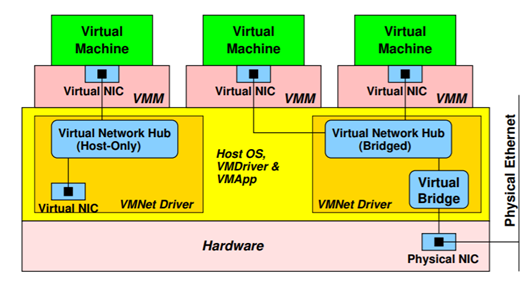
\includegraphics[width=80mm,height=50mm]{virtualizing_network_card.png}
     \caption{Penalty Index Comparison}
     \label{fig:galaxy}
  
 \end{figure}
Reference [1]

[1] Title : Virtualizing I/O Devices on VMware Workstation’s Hosted Virtual Machine Monitor
    Authors: Jeremy Sugerman, Ganesh Venkitachalam and Beng-Hong Lim

\subsection{Network Performance and I/O support}
A hosted virtualization strategy for I/O devices offers excellent flexibility and portability but at a potential tradeoff in performance for high throughput devices. Due to its nature, the hosted architecture incurs the following overheads:\newline

1. A world switch from the VMM to the host is required whenever the virtual machine needs to access real hardware

2. I/O interrupt handling potentially involves the VMM, host OS, and guest OS interrupt handlers

3. A packet transmission by the guest OS involves two device drivers - one in the guest and one on the host there is an extra copy from the guest OS’s physical memory to the host OS’s kernel buffers on a packet transmit.

4. Since these overheads consume CPU cycles, a system that is natively capable of saturating a high performance Ethernet link might instead become CPU bound when run within a virtual machine.


\newline
Currently, I/O device virtualization models in virtual machine (VM) environments
require involvement of a virtual machine monitor (VMM) and/or a privileged VM for
each I/O operation, which may turn out to be a performance bottleneck for systems
with high I/O demands, especially those equipped with modern high speed
interconnects such as InfiniBand.

%



\subsection{Security Issues in VMs} 
The VM is a relatively new project. So, it is quite understandable that it might have some security issues like every other system. As we know VMs are implemented using the hypervisor or VMM technology which acts as a layer between the virtual OS and the underlying hardware. Now, this provides a lot of security features such as isolation, state recording, transience and mobility and External Monitoring. 

Isolation: Isolation refers to the encapsulation of each guest OS and abstraction from the hardware, so that each user accesses separate file systems and memory blocks.

State Recording: The host OS has the ability to record the state of the VM. Most of the VMs take a snapshot of the content changes made in the VM at certain time intervals.

Transience: The VMs have the ability to be created and disabled at any point of time. Thus, the resource management of the underlying system is taken care of by this aspect as the VMs are enabled only when they are required.

Mobility: The VMs created are in the form of an image or a file which can be shared between various systems as a single entity

External Monitoring: They can be monitored from the hypervisor or VM OS dedicated for this purpose.

Security flaws of VMs:
VM Sprawl: The biggest vulnerability of VMs is due to the ease in creation of new Virtual Machines, which makes the monitoring of VMs veryproblematic.

This can also become a serious security flaw if an attacker can restore the state of a Virtual Machine to a previous unsecured one

Title: Hardware-Supported Virtualization on ARM
\begin{figure}[H]
 
      \centering
     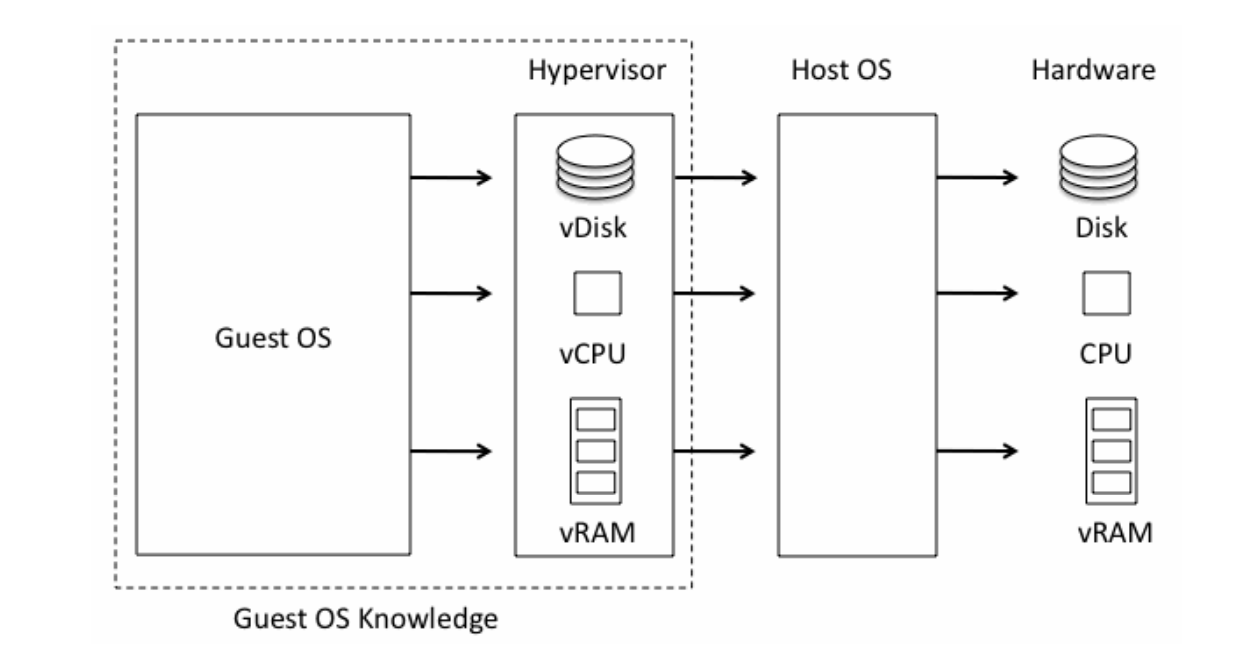
\includegraphics[width=100mm,height=50mm]{guest_os_isolation.png}
     \caption{Penalty Index Comparison}
     \label{fig:galaxy}
  
 \end{figure}


\subsection{MIPS implementation}
MIPS is a ‘typical’ RISC architecture: it has a simple and regular instruction set, only one memory addressing mode (base plus displacement) and instructions are of fixed size (32 bit). MIPS is a register-register (or Load/Store), three address machine. Register-register means that all operations are performed in registers. Access to memory is provided only by load and store instructions. There is no arithmetic or logic instruction. Three-address means that all arithmetic and logic instructions have three operands, one destination register which is always listed immediately after the instruction name, and two source registers.\newline
 
Storage in MIPS
The only way the CPU can access the memory in MIPS is through load and store instructions. There is only one addressing mode (base+displacement). Having just one addressing mode is part of the RISC philosophy to keep instructions simple thus allowing for a simple control structure and efficient pipelining. The kernel space cannot be directly accessed by user programs, and it is reserved for the use of the operating system.

\section{Discussion}
Our main goal in this project was to learn about the technology of Virtual Machine Monitors and how the architectural support is provided to the VM Operating Systems. We all got to learn about the various sub-parts of the Virtual Machine Monitors like how it handles networking, security, I/O control and other important issues, we also identified some bottlenecks and problems in these implementation that exist in the present VM architectures.  


\bibliography{bibliography/first}
\bibliographystyle{splncs04}

[1] Title : Virtualizing I/O Devices on VMware Workstation’s Hosted Virtual Machine Monitor
    Authors: Jeremy Sugerman, Ganesh Venkitachalam and Beng-Hong Lim

Reference 2
[2] Title: Operating System Support for Virtual Machines
    Authors: Samuel T. King, George W. Dunlap, Peter M. Chen

[3] Title : Virtualizing I/O Devices on VMware Workstation’s Hosted Virtual Machine Monitor
    Authors: Jeremy Sugerman, Ganesh Venkitachalam and Beng-Hong Lim

[4] Title: Hardware-Supported Virtualization on ARM
    Authors: Prashant Varanasi, Gernot Heiser

[5] Title: A Survey on the Security of Virtual Machines
    Authors: Doug Hyde
\end{document}